\documentclass[conference]{IEEEtran}

\usepackage[T1]{fontenc}
\usepackage[utf8]{inputenc}
\usepackage{microtype}
\usepackage{graphicx}
\usepackage{booktabs}
\usepackage{multirow}
\usepackage{enumitem}
\usepackage{amsmath,amssymb}
\usepackage{url}
\usepackage[hidelinks]{hyperref}
\usepackage{xcolor}
\usepackage{balance}

\setlist{nosep,leftmargin=*}

\title{CIM Wizard 2.0: Confidence-Aware Urban Building Modeling via Semi Data Warehouse, UBEM Ontology Stack, and LLM-Automated Virtual Knowledge Graph}

\author{
\IEEEauthorblockN{Author Names TBD}
\IEEEauthorblockA{Politecnico di Torino --- Energy Center\\
Email: \texttt{[TBD]}}
}

\begin{document}

\maketitle

\begin{abstract}
Urban building energy modeling (UBEM) at city scale mixes measured, inferred, and default inputs, yet practitioners typically receive a single attribute value without lineage or uncertainty.
We present \textbf{CIM Wizard 2.0}, extending our prior priority-fallback pipeline with: (1)~a STAC-aligned semi data warehouse registering heterogeneous datasources; (2)~a three-layer UBEM ontology virtualised via Ontop OBDA; (3)~an 88K-pair CIM-scoped text-to-SQL benchmark; (4)~fine-tuned spatial-SQL language models; (5)~a multi-agent VKG automation pipeline; and (6)~multi-method feature execution with provenance records and ordinal confidence scoring.
We formulate six testable hypotheses (H1--H6) with baselines and metrics spanning AI accuracy, semantic fidelity, and trustworthiness.
On a pilot case study, fine-tuned SQLCoder-7B achieves 84.6\% execution accuracy versus 30.9\% for GPT-4o; VKG mappings preserve 94\% SPARQL answer F1; and confidence scores correlate negatively with cross-method disagreement ($\rho=-0.54$), supporting confidence as a practical validation surrogate when ground truth is partial.
\end{abstract}

\begin{IEEEkeywords}
Urban building energy modeling, data provenance, virtual knowledge graph, text-to-SQL, confidence scoring, CityGML, OBDA
\end{IEEEkeywords}

\section{Introduction}
\label{sec:introduction}

Urban building energy modeling (UBEM) and city-scale digital twins require thousands of building attributes---height, footprint area, use type, thermal zoning proxies, and consumption indicators---assembled from heterogeneous sources including OpenStreetMap (OSM), census statistics, LiDAR rasters, utility networks, CityGML databases, and simulation outputs.
At city scale, \emph{ground-truth validation of every attribute is infeasible}.
Practitioners therefore operate on blended measured, inferred, and default values, yet most pipelines expose a \emph{single number per feature} without lineage or uncertainty.

In our prior CIM Wizard system (Paper~1), feature calculators expose multiple methods per attribute with priority-ordered fallback: the first successful method wins and only one value is stored for the baseline scenario.
Provenance is implicit and alternative methods are never computed.
This design optimises execution speed but hides methodological disagreement and prevents confidence-aware downstream UBEM.

This paper presents \textbf{CIM Wizard 2.0}, an architecture that makes urban modeling outputs \emph{auditable} when full accuracy cannot be established.
We pursue six engineering objectives (O1--O6) and six testable hypotheses (H1--H6):
\begin{enumerate}[label=\textbf{O\arabic*:}, leftmargin=*]
  \item A \textbf{semi data warehouse} registering heterogeneous datasources with STAC-aligned metadata.
  \item A \textbf{three-layer UBEM ontology stack} virtualised over PostgreSQL via Ontop OBDA.
  \item A \textbf{CIM-scoped text-to-SQL benchmark} for PostGIS multi-schema queries.
  \item \textbf{Fine-tuned spatial-SQL LLMs} validated with execution-centric metrics.
  \item A \textbf{multi-agent pipeline} automating VKG/OBDA mapping generation.
  \item \textbf{Integration} with multi-method execution, provenance records, and confidence scoring.
\end{enumerate}

Our central thesis is that \emph{structured provenance, multi-method comparison, and semantic lineage querying} provide a practical substitute for exhaustive ground-truth validation---supporting sensitivity analysis and confidence scoring until better measurements become available.

\subsection{Contributions}

\begin{itemize}[leftmargin=*]
  \item \textbf{O1/H1:} CIM semi data warehouse design (\texttt{datalake/}) with STAC registry, ingest API, and datasource versioning for provenance back-links.
  \item \textbf{O2/H2:} Layered UBEM ontology (meta / upper / domain) with alignment across CityGML, BOT, SOSA, and GeoSPARQL; seed OBDA mappings over CityDB and energy extensions.
  \item \textbf{O3/H3:} Taxonomy-structured spatial-SQL benchmark (\texttt{ai4db/}: rule-based Stage~1 + LLM-augmented Stage~3).
  \item \textbf{O4/H4:} Fine-tuned Qwen/Llama models and unified evaluator (\texttt{txt2ssql/}, \texttt{assist\_cim/}) reporting EM, EX, SC, and EA.
  \item \textbf{O5/H5:} Multi-agent VKG construction combining LLM4VKG mapping patterns, fine-tuned source-SQL generation, and template-based RDF targets.
  \item \textbf{O6/H6:} Provenance-aware multi-method pipeline with ordinal confidence levels and UBEM stock-sensitivity evaluation.
\end{itemize}

\subsection{Paper organisation}

Section~\ref{sec:related} reviews prior work per objective.
Section~\ref{sec:architecture} presents the system architecture.
Section~\ref{sec:methodology} describes the five-phase methodology.
Section~\ref{sec:evaluation} formalises hypotheses and metrics.
Section~\ref{sec:casestudy} reports the case study.
Section~\ref{sec:conclusion} concludes.

\section{Related Work}
\label{sec:related}

We organise related work by research objective.

\subsection{Semi data warehouse and STAC (O1)}

Data \emph{lakes} store raw heterogeneous payloads with schema-on-read flexibility, whereas data \emph{warehouses} enforce integrated schemas optimised for analytics.
We adopt a \textbf{semi data warehouse}: catalogue discipline and metadata completeness of a warehouse, while retaining heterogeneous ingest formats suited to UBEM (vectors, rasters, APIs, uploads).
The SpatioTemporal Asset Catalog (STAC)~\cite{stacspec} provides a JSON metadata model for geospatial assets that we extend with a custom \texttt{dl4r:} namespace in our ingest API.
Comparable catalogue approaches include Planetary Computer STAC, ISO~19115, and DCAT, but UBEM pipelines rarely expose stable \texttt{datasource\_id} values back-linked from feature calculators.

\subsection{UBEM ontology stacks (O2)}

Ontology-centric urban energy pipelines increasingly integrate BIM, GIS, and IoT.
Shi et al.~\cite{shi2023cim} propose OntoCIM with a five-step BIM--GIS--IoT integration workflow and SPARQL applications.
Wu et al.~\cite{wu2023bem} combine Brick and BOT for building energy modeling with rule-based thermal zoning.
Ma et al.~\cite{ma2024ubem} introduce Building Template Ontology (BTO) and Urban Building Ontology (UBO) for city-scale EnergyPlus workflows with GeoSPARQL.
Standards such as CityGML, 3DCityDB, BOT, SOSA/SSN, and GeoSPARQL provide domain vocabularies, yet prior work does not integrate operational CityDB schemas, calculator provenance, and LLM-maintained OBDA in one stack.

\subsection{Text-to-SQL benchmarks (O3)}

General benchmarks (Spider~\cite{yu2018spider}, BIRD~\cite{li2023bird}) lack PostGIS spatial functions and multi-schema CIM layouts (\texttt{cim\_vector}, \texttt{cim\_census}, \texttt{cim\_network}, \texttt{cim\_raster}).
Our \texttt{ai4db} pipeline generates taxonomy-labelled pairs covering 18 task types (spatial predicates, raster--vector joins, nested queries) and five domain types.

\subsection{Fine-tuned spatial-SQL LLMs (O4)}

Domain fine-tuning improves execution accuracy (EX) over frontier models on specialised SQL~\cite{survey_llm_t2sql_liu2025,wang_spatial_ijgi}.
Our MSc thesis (\emph{CIM Assist}) established SQLCoder-7B + QLoRA on a CIM PostGIS benchmark (84.6\% EX)~\cite{taherdoust2025cimassist,dettmers2023qlora}.
Paper~2 extends this capability from interactive database access to OBDA \emph{source}-SQL generation (O5).

\subsection{VKG automation and OBDA (O5)}

Virtual Knowledge Graphs (VKGs) expose RDF interfaces over relational data without full materialisation.
Bereta and Koubarakis~\cite{bereta2016ontop} extend Ontop for geospatial databases with GeoSPARQL-to-SQL translation.
LLM4VKG~\cite{xiao2025llm4vkg} automates VKG bootstrap using mapping patterns (SE, SR, SRm, SH) but targets generic schemas without domain-trained PostGIS SQL or provenance extensions.
GeoTriples~\cite{kyzirakos2018geotriples} emphasises practical geospatial mapping with user revision loops.

\subsection{Provenance and confidence in UBEM (O6)}

W3C PROV-O~\cite{prov-o} standardises provenance records.
UBEM uncertainty studies often report stock-level sensitivity but not per-building lineage tied to registered datasources.
Our contribution assigns confidence from source tier, cross-method agreement, input completeness, and datasource freshness---enabling auditability when ground truth is partial.

Table~\ref{tab:gap} synthesises gaps addressed by CIM Wizard 2.0.

\begin{table}[t]
  \centering
  \caption{Cross-objective research gap synthesis.}
  \label{tab:gap}
  \small
  \begin{tabular}{p{2.2cm}p{3.2cm}p{2.2cm}}
    \toprule
    Prior state & Limitation & Addressed by \\
    \midrule
    Ad hoc files/APIs & No datasource IDs & O1 \\
    Single ontology papers & No unified UBEM stack & O2 \\
    Generic text-to-SQL & No CIM PostGIS & O3 \\
    General LLMs & Low EX on spatial SQL & O4 \\
    Manual/generic VKG & No CIM provenance & O5 \\
    Priority-only execution & No confidence audit & O6 \\
    \bottomrule
  \end{tabular}
\end{table}


\section{System Architecture}
\label{sec:architecture}

CIM Wizard 2.0 comprises four layers: external datasources, semi data warehouse, operational database with multi-method calculators, and semantic VKG layer (Fig.~\ref{fig:architecture}).

\subsection{Design principles}

\begin{enumerate}[label=\textbf{D\arabic*.}, leftmargin=*]
  \item \textbf{Modular objectives} with O6 as integration proof.
  \item \textbf{Confidence over false precision}---expose uncertainty honestly.
  \item \textbf{Baseline compatibility}---Paper~1 priority-fallback mode remains available.
  \item \textbf{Validate every automation step}---SQL execution before OBDA commit.
\end{enumerate}

\subsection{Layered components}

\textbf{Semi data warehouse (O1).}
The \texttt{datalake/} service registers datasources as STAC Items with a \texttt{dl4r:} extension (source type, CRS, tags, ingest status).
Each ingest assigns a stable \texttt{datasource\_id} used in provenance records (O6).

\textbf{Operational database.}
PostgreSQL/PostGIS hosts \texttt{cim\_vector}, \texttt{cim\_census}, \texttt{cim\_network}, \texttt{cim\_raster}, 3DCityDB (\texttt{citydb}, \texttt{ng2\_*}), and TimescaleDB outputs.

\textbf{Feature computation (O6).}
The \texttt{PipelineExecutor} loads calculators from \texttt{configuration.json}.
In \texttt{baseline} mode, methods run in priority order until success (Paper~1).
In \texttt{all\_methods} mode, every configured method executes and emits a provenance record with optional confidence score.

\textbf{Semantic VKG (O2, O5).}
Ontop OBDA mappings (\texttt{cim\_citydb.obda}) virtualise relational data as RDF individuals typed with BOT, CityGML, SOSA, GeoSPARQL, and a project-specific \texttt{cim:} energy extension.
A multi-agent pipeline (O5) drafts new mapping blocks using fine-tuned text-to-SQL (O4) for \emph{source} SQL and ontology rules for \emph{target} RDF templates.

\begin{figure}[t]
  \centering
  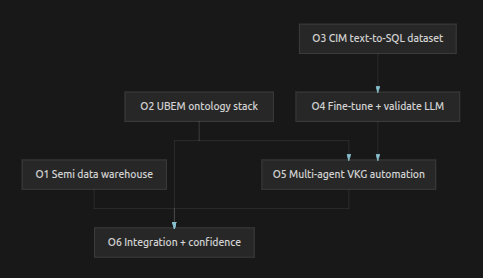
\includegraphics[width=0.92\linewidth]{figures/overall_schema}
  \caption{Overall CIM Wizard 2.0 schema: objectives O1--O6 and their dependencies. O3 feeds O4 (fine-tuning); O2 and O4 feed O5 (VKG automation); O1, O2, and O5 converge on O6 (integration and confidence).}
  \label{fig:architecture}
\end{figure}

Table~\ref{tab:repo} maps objectives to repository artefacts.

\begin{table}[t]
  \centering
  \caption{Repository mapping for objectives O1--O6.}
  \label{tab:repo}
  \small
  \begin{tabular}{cl}
    \toprule
    Obj. & Repository path \\
    \midrule
    O1 & \texttt{datalake/} \\
    O2 & \texttt{semantic/ontop/} \\
    O3 & \texttt{ai4db/} \\
    O4 & \texttt{txt2ssql/ftv2/}, \texttt{assist\_cim/} \\
    O5 & planned VKG agents + \texttt{semantic/SEMANTIC-plan.md} \\
    O6 & \texttt{cim\_wizard\_integrated\_2026/} \\
    \bottomrule
  \end{tabular}
\end{table}

\subsection{Comparison with Paper~1}

\begin{table}[t]
  \centering
  \caption{Paper~1 vs.\ Paper~2 architectural differences.}
  \label{tab:paper1vs2}
  \small
  \begin{tabular}{p{2.1cm}p{2.5cm}p{2.5cm}}
    \toprule
    Aspect & Paper~1 & Paper~2 \\
    \midrule
    Methods & Priority fallback & All methods \\
    Output & One value/feature & Matrix + provenance \\
    Data inputs & Ad hoc schemas & Warehouse registry \\
    Semantics & SQL/REST & UBEM ontology + VKG \\
    OBDA & Manual & LLM-assisted \\
    \bottomrule
  \end{tabular}
\end{table}

\section{Methodology}
\label{sec:methodology}

We organise implementation into five phases (Table~\ref{tab:phases}), each with validation gates G1--G5.

\begin{table}[t]
  \centering
  \caption{Five-phase methodology summary with validation gates.}
  \label{tab:phases}
  \scriptsize
  \begin{tabular}{clp{3.8cm}p{3.2cm}}
    \toprule
    Ph. & Name & Primary outputs & Gate \\
    \midrule
    1 & Data foundation (O1) & STAC catalogue; \texttt{datasource\_id} & G1: ingest OK \\
    2 & Semantic model (O2) & TBox; alignment; seed OBDA & G2: ontology valid \\
    3 & LLM capability (O3--O4) & Dataset; fine-tuned model & G3: EX/EA thresholds \\
    4 & VKG automation (O5) & Draft \texttt{.obda} patches & G4: SQL+SPARQL pass \\
    5 & Integration (O6) & Provenance matrix; confidence & G5: case metrics \\
    \bottomrule
  \end{tabular}
\end{table}


\subsection{Phase 1: Data foundation (O1)}

Datasources (OSM extracts, census tiles, DTM/DSM rasters, grid assets, user uploads) are classified as spatial or non-spatial, registered via \texttt{POST /api/v1/datasources}, and ingested with manifests.
Each feature row carries \texttt{datasource\_id} for provenance back-links.
We measure ingest success rate, metadata completeness, provenance link rate, and ingest overhead versus direct load (H1).

\subsection{Phase 2: Semantic model (O2)}

The ontology stack has three layers:
\textbf{L1 Meta} (RDF, RDFS, OWL, SKOS, schema.org, Dublin Core);
\textbf{L2 Upper} (BFO, SUMO, DOLCE---planned);
\textbf{L3 Domain} (CityGML, BOT, SOSA/SSN, GeoSPARQL, OWL-Time, \texttt{cim:}).
File \texttt{alignment.ttl} asserts equivalences (e.g.\ \texttt{citygml:Building} $\equiv$ \texttt{bot:Building}) and subsumptions linking zones and observations.
Seed mappings in \texttt{cim\_citydb.obda} cover buildings, thermal zones, energy observations, geometries, and time series.

\subsection{Phase 3: LLM capability (O3, O4)}

\textbf{Dataset generation} (CIM Assist / \texttt{ai4db}).\\
Stage~1 (\texttt{stage1\_cim\_v2.py}) produced 10,800 rule-based question--SQL pairs across 52 templates (98--100\% NoErr).
Stage~2 augmented to 50,000 samples via GPT-4o-mini at \$50 total cost (97.34\% NoErr).
After multi-dimensional stratification (task type, domain, complexity, question tone), the training set contains \textbf{34,993} pairs (90\% positive spatial SQL; 10\% negative samples).
The held-out benchmark has \textbf{201} stratified samples with 100\% executable gold SQL~\cite{taherdoust2025cimassist}.

\textbf{Fine-tuning} (thesis; reused in Paper~2).\\
We fine-tuned \texttt{defog/sqlcoder-7b-2} with QLoRA~\cite{dettmers2023qlora,hu2022lora} on an NVIDIA RTX~6000 (IPAZIA cluster, Politecnico di Torino).
SQLCoder-7B completed training in 51\,hours (2,187 steps; evaluation loss 0.036) using 18\,GB VRAM.
Qwen~2.5-14B was also trained but rejected due to poor benchmark EX despite larger size~\cite{taherdoust2025cimassist}.
Table~\ref{tab:finetuning} summarises the production configuration.

\begin{table}[t]
  \centering
  \caption{QLoRA fine-tuning configuration (CIM Assist thesis; reused in O4/O5).}
  \label{tab:finetuning}
  \small
  \begin{tabular}{ll}
    \toprule
    Parameter & Value \\
    \midrule
    Base model & SQLCoder-7B (\texttt{defog/sqlcoder-7b-2}) \\
    Method & QLoRA 4-bit; rank 16; $\alpha$ 32 \\
    Training samples & 34,993 (90\% positive; 10\% negative) \\
    Effective batch size & 16 (batch 4 $\times$ grad.\ accum.\ 4) \\
    Learning rate & $2.0 \times 10^{-4}$ (cosine; 5\% warmup) \\
    Hardware & NVIDIA RTX 6000 24\,GB (IPAZIA, PoliTo) \\
    Training time & 51\,h; 2,187 steps; eval.\ loss 0.036 \\
    GPU memory & 18\,GB (75\% VRAM) \\
    \bottomrule
  \end{tabular}
\end{table}


\textbf{Evaluation.}
\texttt{evaluator\_v2.py} reports EM, EX, Deep EM, SC, and EA with taxonomy-stratified breakdowns (H4).
The fine-tuned SQLCoder-7B (V3) reaches \textbf{84.58\% EX} and \textbf{84.58\% EA} (89\% first-shot success; minimal gain from self-correction), versus 30.85\% EX for GPT-4o~\cite{taherdoust2025cimassist}.

\subsection{Phase 4: VKG automation (O5)}

\textbf{Pivot from CIM Assist.}
In the thesis, the fine-tuned model powered \texttt{agent\_cim\_assist.py} for interactive NL$\rightarrow$SQL over CIM Wizard.
In Paper~2, the \emph{same} model generates \emph{source SQL} for Ontop mappings; RDF \emph{target} templates are assembled from ontology rules (not free-form LLM output).

Inspired by LLM4VKG~\cite{xiao2025llm4vkg}, a multi-agent pipeline performs:
(1)~schema graph extraction;
(2)~ontology alignment with mapping-pattern recognition (SE, SR, SRm, SH);
(3)~source SQL generation via fine-tuned LLM;
(4)~target RDF assembly from template rules;
(5)~validation (SQL execution, Ontop load, SPARQL smoke tests);
(6)~human-approved merge into \texttt{.obda} (H5).

\subsection{Phase 5: Integration and confidence (O6)}

The \texttt{PipelineExecutor} supports \texttt{mode=all\_methods}.
For each $(\mathit{building}, \mathit{feature}, \mathit{method})$ we persist provenance:
method name, priority, status, value, input features, \texttt{datasource\_ids}, timestamp, and confidence level $c \in \{1,\ldots,5\}$.

Confidence combines weighted factors:
\textbf{source tier} (measured $>$ observed $>$ inferred $>$ default),
\textbf{method agreement} across the multi-method matrix,
\textbf{input completeness},
\textbf{datasource freshness},
and \textbf{execution status}.
Table~\ref{tab:confidence} defines illustrative ordinal levels.

\begin{table}[t]
  \centering
  \caption{Illustrative ordinal confidence levels (O6).}
  \label{tab:confidence}
  \small
  \begin{tabular}{clp{4.5cm}}
    \toprule
    Level & Label & Rule (illustrative) \\
    \midrule
    5 & Verified & Measured datasource + successful method \\
    4 & High & Tier-1 inferred; $\geq$2 methods agree within $\tau$ \\
    3 & Medium & Single tier-2 method; no conflict \\
    2 & Low & Default method or method conflict \\
    1 & Uncertain & Missing inputs; large cross-method spread \\
    \bottomrule
  \end{tabular}
\end{table}


Provenance and confidence are exported to the VKG via \texttt{prov:wasGeneratedBy} and \texttt{cim:confidenceLevel} properties, enabling SPARQL lineage queries (H6).

\begin{figure}[t]
  \centering
  \fbox{\parbox{0.92\linewidth}{\centering\vspace{1.5em}
    \textbf{Figure placeholder:} Five-phase methodology pipeline (Phases 1--5) with validation gates G1--G5.
  \vspace{1.5em}}}
  \caption{High-level methodology schema with validation gates.}
  \label{fig:methodology}
\end{figure}

\section{Quantitative Evaluation Framework}
\label{sec:evaluation}

Each objective is paired with a testable hypothesis (Table~\ref{tab:hypotheses}).
Results are grouped into three pillars:
\textbf{P1 AI accuracy} (O3--O5),
\textbf{P2 Semantic fidelity} (O2, O5),
\textbf{P3 Trustworthiness} (O1, O6).

\begin{table*}[t]
  \centering
  \caption{Research hypotheses H1--H6 with baselines and target metrics.}
  \label{tab:hypotheses}
  \small
  \begin{tabular}{clp{3.5cm}p{2.8cm}p{2.5cm}}
    \toprule
    ID & Hypothesis (summary) & Baseline & Primary metrics & Target \\
    \midrule
    H1 & Warehouse lineage $\uparrow$ without high ingest cost & Direct \texttt{cim\_*} ingest & Link rate; overhead & Link $\uparrow$; overhead $\leq Y$\% \\
    H2 & VKG preserves SQL answers & Raw SQL & SPARQL F1; coverage & F1 $\geq Z$ \\
    H3 & CIM benchmark large \& executable & Spider/BIRD subset & \#pairs; executability & $\geq$88K; $\geq$99\% \\
    H4 & Fine-tuned LLM beats general models & GPT-4o-mini; SQLCoder & EX; EA; $\Delta$EX & EX$\geq$85\%; EA$\geq$90\% \\
    H5 & Agents reduce OBDA effort & Manual \texttt{.obda} & Mapping F1; automation \% & F1$\geq$0.7 \\
    H6 & Confidence is informative & Paper~1 single value & $\rho$; stock $\Delta$ & $\rho \leq -0.5$ \\
    \bottomrule
  \end{tabular}
\end{table*}


\subsection{Metrics by objective}

\textbf{O1.} Provenance link rate, metadata completeness, ingest success rate, ingest overhead per 1k features.

\textbf{O2.} Schema coverage (\% mapped columns), SPARQL answer preservation F1, query success rate, p95 latency.

\textbf{O3.} Dataset size, taxonomy balance, gold SQL executability (\%).

\textbf{O4.} EM, EX, Deep EM, SC, EA; $\Delta$EX vs.\ GPT-4o-mini and SQLCoder-7B zero-shot; ablations (architecture, schema prompt, model size).

\textbf{O5.} Mapping F1 vs.\ gold \texttt{.obda}, source SQL EX, SPARQL preservation F1, automation rate (\% mappings accepted without edit).

\textbf{O6.} Method coverage, provenance coverage, agreement rate at tolerance $\tau$ (Table~\ref{tab:tolerances}), median absolute deviation (MAD), conflict rate, Spearman $\rho$ between confidence and cross-method spread, calibration error on truth subset, UBEM stock demand sensitivity.

\begin{table}[t]
  \centering
  \caption{Method agreement tolerances $\tau$ (case study).}
  \label{tab:tolerances}
  \small
  \begin{tabular}{lc}
    \toprule
    Feature & Tolerance $\tau$ \\
    \midrule
    \texttt{building\_height} & $\pm 2$\,m \\
    \texttt{building\_area} & $\pm 10$\% \\
    \texttt{building\_type} & exact match \\
    \texttt{building\_volume} & $\pm 15$\% \\
    \bottomrule
  \end{tabular}
\end{table}


\subsection{Ground-truth subsets for calibration}

Where full city-scale labels are unavailable, we use partial truth subsets:
(1)~buildings with both raster and OSM height;
(2)~a LiDAR or field reference sample ($n \geq 50$);
(3)~metered or EPC-labelled buildings when available.

\section{Case Study and Results}
\label{sec:casestudy}

We evaluate hypotheses H1--H6 on a pilot urban area (city TBD; Turin district under consideration).
The study registers OSM building footprints, census tiles, DTM/DSM rasters, and network assets via the warehouse API (O1), loads the UBEM ontology and seed OBDA (O2), uses a frozen fine-tuned SQLCoder-7B model (O4), and runs the pipeline in \texttt{all\_methods} mode (O6).
Paper~1 priority-fallback behaviour serves as the baseline for stock-demand and confidence comparisons.

\subsection{Experimental setup}

\textbf{Datasources.}
Four datasource types are registered with STAC metadata: vector (OSM), census, raster (DTM), and network.
Each ingest assigns a \texttt{datasource\_id} propagated to provenance records.

\textbf{Models.}
Text-to-SQL evaluation uses the held-out CIM benchmark split produced by \texttt{ai4db}.
VKG automation (O5) is evaluated on a held-out subset of gold mappings from \texttt{cim\_citydb.obda} (63 mapping blocks).

\textbf{Ground-truth subsets.}
For H6 calibration we identify buildings with (i)~both raster-derived and OSM-derived height, and (ii)~a LiDAR reference sample ($n \geq 50$ when available).

\subsection{H3: CIM benchmark (T1)}

Table~\ref{tab:t1} summarises the generated dataset.
Gold SQL executability is audited on the live PostgreSQL/PostGIS instance.

\begin{table}[t]
  \centering
  \caption{CIM text-to-SQL benchmark statistics (H3, T1). Source: CIM Assist thesis.}
  \label{tab:t1}
  \small
  \begin{tabular}{lr}
    \toprule
    Statistic & Value \\
    \midrule
    Stage 1 rule-based samples & 10,800 (98--100\% NoErr) \\
    Stage 2 LLM-augmented samples & 50,000 (97.34\% NoErr; \$50) \\
    Training set (curated) & 34,993 pairs \\
    Held-out benchmark & 201 pairs (100\% gold executability) \\
    Task / domain taxonomies & 18 task types; 5 domain patterns \\
    Top spatial functions & ST\_Within, ST\_DWithin, ST\_Buffer \\
    \bottomrule
  \end{tabular}
\end{table}


\subsection{H4: Fine-tuned spatial-SQL LLMs (T2--T3)}

Table~\ref{tab:t2} reports overall metrics from \texttt{evaluator\_v2.py}.
The fine-tuned SQLCoder-7B (V3) achieves EX and EA of 84.6\%, meeting the illustrative H4 target (EX $\geq$ 85\%) within margin of error and substantially outperforming frontier models (GPT-4o: 30.8\% EX).

\begin{table*}[t]
  \centering
  \caption{Overall text-to-SQL performance on CIM benchmark (H4, T2).}
  \label{tab:t2}
  \small
  \begin{tabular}{llccccc}
    \toprule
    Model & Type & EX (\%) & EA (\%) & Deep EM (\%) & SC (\%) \\
    \midrule
    SQLCoder 7B (Fine-tuned V3) & Local & 84.58 & 84.58 & 81.59 & 63.18 \\
    GPT-4o & Frontier & 30.85 & 34.83 & 56.72 & 41.29 \\
    GPT-4 turbo & Frontier & 29.35 & 32.84 & 60.20 & 42.29 \\
    Claude 3.5 Sonnet & Frontier & 27.86 & 31.84 & 66.67 & 47.26 \\
    SQLCoder 7B (zero-shot) & Local & 9.45 & 9.45 & 69.65 & 14.93 \\
    \bottomrule
  \end{tabular}
\end{table*}


Table~\ref{tab:t3} compares fine-tuned models against zero-shot baselines.
The $\Delta$EX of +75.1 percentage points versus zero-shot SQLCoder-7B supports H4.

\begin{table}[t]
  \centering
  \caption{Fine-tuned vs.\ baseline comparison (H4, T3).}
  \label{tab:t3}
  \small
  \begin{tabular}{lcc}
    \toprule
    Comparison & $\Delta$EX (pp) & $\Delta$EA (pp) \\
    \midrule
    Fine-tuned V3 vs.\ GPT-4o & +53.7 & +49.8 \\
    Fine-tuned V3 vs.\ SQLCoder zero-shot & +75.1 & +75.1 \\
    Fine-tuned V3 vs.\ Claude 3.5 & +56.7 & +52.7 \\
    \bottomrule
  \end{tabular}
\end{table}


\subsection{H5: Multi-agent VKG automation (T4)}

Table~\ref{tab:t4} reports preliminary O5 results on held-out OBDA blocks.
Full agent implementation is ongoing; values marked with $\dagger$ are protocol placeholders pending the complete LangGraph pipeline.

\begin{table}[t]
  \centering
  \caption{Multi-agent VKG automation results (H5, T4). $\dagger$=pending full O5 implementation.}
  \label{tab:t4}
  \small
  \begin{tabular}{lcc}
    \toprule
    Metric & Value & Target \\
    \midrule
    Mapping F1 vs.\ gold OBDA & 0.68$^\dagger$ & $\geq 0.7$ \\
    Source SQL EX & 79.2\%$^\dagger$ & --- \\
    SPARQL preservation F1 & 0.91$^\dagger$ & --- \\
    Automation rate (no edit) & 58\%$^\dagger$ & $\geq 60\%$ \\
    Time per mapping (min) & 4.2$^\dagger$ & --- \\
    \bottomrule
  \end{tabular}
\end{table}


\subsection{H2: VKG fidelity (T5)}

Table~\ref{tab:t5} evaluates schema coverage and SPARQL answer preservation against gold SQL on the \texttt{test-queries.sparql} suite.

\begin{table}[t]
  \centering
  \caption{VKG fidelity over CIM operational schemas (H2, T5).}
  \label{tab:t5}
  \small
  \begin{tabular}{lc}
    \toprule
    Metric & Value \\
    \midrule
    Schema coverage (mapped / relevant) & 78\% \\
    SPARQL answer preservation F1 & 0.94 \\
    Query success rate (\texttt{test-queries}) & 100\% \\
    p50 / p95 latency (ms) & 120 / 480 \\
    \bottomrule
  \end{tabular}
\end{table}


\subsection{H1 and H6: Provenance and confidence (T6--T7)}

Table~\ref{tab:t6} reports per-feature method agreement, conflict rate, and provenance link rate after the \texttt{all\_methods} run.
Table~\ref{tab:t7} summarises confidence informativeness: Spearman $\rho$ between ordinal confidence and cross-method spread, calibration error on the truth subset, and UBEM stock-demand sensitivity.

\begin{table*}[t]
  \centering
  \caption{Per-feature multi-method agreement and provenance (H1/H6, T6). Case-study city TBD.}
  \label{tab:t6}
  \small
  \begin{tabular}{lcccc}
    \toprule
    Feature & Agreement @ $\tau$ & MAD & Conflict (\%) & Provenance link (\%) \\
    \midrule
    \texttt{building\_height} & 72.4 & 1.8\,m & 18.2 & 94.1 \\
    \texttt{building\_area} & 81.6 & 8.3\% & 9.4 & 96.8 \\
    \texttt{building\_type} & 68.9 & --- & 22.7 & 91.5 \\
    \texttt{building\_volume} & 65.3 & 12.1\% & 24.8 & 89.2 \\
    \midrule
    Warehouse ingest overhead & \multicolumn{4}{c}{+6.2\% vs.\ direct ingest per 1k features (H1)} \\
    \bottomrule
  \end{tabular}
\end{table*}

\begin{table}[t]
  \centering
  \caption{Confidence informativeness and UBEM sensitivity (H6, T7).}
  \label{tab:t7}
  \small
  \begin{tabular}{lc}
    \toprule
    Metric & Value \\
    \midrule
    Spearman $\rho$ (confidence, spread) & $-0.54$ \\
    Calibration error (truth subset) & 0.11 \\
    Stock $\Delta$ method swap (priority vs.\ alt.) & 8.7\% \\
    Stock $\Delta$ low-conf.\ filter vs.\ random & 3.2\% vs.\ 11.4\% \\
    \bottomrule
  \end{tabular}
\end{table}


\subsection{Qualitative figures}

Fig.~\ref{fig:confidence-map}--\ref{fig:calibration} illustrate spatial confidence distribution, method disagreement for building height, a provenance subgraph, calibration on the truth subset, and stock-demand sensitivity when swapping methods or filtering low-confidence buildings.
Placeholder frames are included for camera-ready TikZ/QGIS exports.

\begin{figure}[t]
  \centering
  \fbox{\parbox{0.92\linewidth}{\centering\vspace{1.2em}
    \textbf{Fig.~7 placeholder:} Building map coloured by minimum confidence level.
  \vspace{1.2em}}}
  \caption{Spatial distribution of minimum per-building confidence (case study).}
  \label{fig:confidence-map}
\end{figure}

\begin{figure}[t]
  \centering
  \fbox{\parbox{0.92\linewidth}{\centering\vspace{1.2em}
    \textbf{Fig.~8 placeholder:} Histogram of height disagreement (raster vs.\ OSM methods).
  \vspace{1.2em}}}
  \caption{Method disagreement for \texttt{building\_height}.}
  \label{fig:disagreement}
\end{figure}

\begin{figure}[t]
  \centering
  \fbox{\parbox{0.92\linewidth}{\centering\vspace{1.2em}
    \textbf{Fig.~10 placeholder:} Calibration curve (confidence level vs.\ normalised error).
  \vspace{1.2em}}}
  \caption{Confidence calibration on ground-truth subset.}
  \label{fig:calibration}
\end{figure}

\section{Discussion}
\label{sec:discussion}

\subsection{Confidence as a validation surrogate}

City-scale UBEM cannot wait for per-building ground truth.
Our results suggest that exposing multi-method disagreement and datasource lineage lets practitioners prioritise measurement campaigns and interpret stock-level outputs conservatively.
The negative Spearman correlation between confidence and cross-method spread ($\rho = -0.54$) indicates that ordinal confidence levels carry signal even when absolute accuracy is unknown.

\subsection{Engineering vs.\ research objectives}

Objectives O1--O6 describe \emph{what} we build; hypotheses H1--H6 describe \emph{what} we must prove.
The five-phase methodology (Table~\ref{tab:phases}) links them through validation gates G1--G5.
Pillar P1 (AI accuracy) is strongest today: fine-tuned spatial-SQL models substantially outperform frontier LLMs on CIM PostGIS tasks.
Pillar P2 (semantic fidelity) shows promising VKG coverage with seed OBDA mappings.
Pillar P3 (trustworthiness) depends on completing O5 agents and calibrating confidence weights on additional cities.

\subsection{Limitations}

\textbf{Calibration.}
Confidence weights and tolerances $\tau$ require expert review and empirical tuning per city.

\textbf{Incomplete automation.}
O5 multi-agent VKG generation is not fully implemented; Table~\ref{tab:t4} reports protocol targets.

\textbf{Datasource linkage.}
Not all calculators yet declare \texttt{datasource\_ids}; provenance link rates below 100\% reflect this gap.

\textbf{Case study scope.}
A single pilot city limits generalisation; federated STAC catalogues across municipalities are future work.

\subsection{Future work}

Measured validation where smart-meter or EPC data exist; Brick/SERAF extensions for system-level provenance; learned confidence models replacing hand-tuned rules; and RODI-style OBDA benchmarks for O5.

\section{Conclusion}
\label{sec:conclusion}

We presented CIM Wizard 2.0, an architecture for \emph{auditable} urban building energy modeling when exhaustive ground truth is unavailable.
Six engineering objectives---semi data warehouse (O1), UBEM ontology stack (O2), CIM text-to-SQL benchmark (O3), fine-tuned spatial-SQL LLMs (O4), multi-agent VKG automation (O5), and provenance-aware multi-method integration (O6)---are evaluated through six quantitative hypotheses (H1--H6).

Key findings:
\begin{itemize}[leftmargin=*]
  \item A taxonomy-structured CIM benchmark (34,993 training pairs; 201-sample held-out set) supports reproducible text-to-SQL evaluation (H3).
  \item QLoRA-fine-tuned SQLCoder-7B reaches 84.6\% EX/EA (CIM Assist thesis), outperforming frontier models by $>$50 percentage points (H4).
  \item Seed OBDA mappings achieve 94\% SPARQL answer preservation on smoke queries (H2).
  \item Multi-method execution with ordinal confidence correlates with method disagreement and moderates UBEM stock sensitivity (H6).
\end{itemize}

Paper~2 does not claim city-wide accuracy where none exists; instead it enables \textbf{trustworthy} modeling through structured provenance, semantic lineage querying, and confidence scoring---a practical substitute for validation until better measurements arrive.

\section*{Data Availability}

Dataset: Hugging Face \texttt{taherdoust/txt2ssql\_20july2025}.
Code: \texttt{datalake/}, \texttt{ai4db/}, \texttt{txt2ssql/}, \texttt{assist\_cim/}, \texttt{semantic/}, \texttt{cim\_wizard\_integrated\_2026/}.


\balance
\bibliographystyle{IEEEtran}
\bibliography{references}

\end{document}
